\chapter{Approach}

In this chapter, the work towards modeling a moving human is described. Starting out, there was much to be figured out and tried. Many questions were not only unanswered but still unasked. The target was already defined: a rigged 3D mesh of the user. The tools available were a Microsoft Kinect for Xbox 360 and a desktop computer.

\section{Obtaining point cloud data}

The first step towards achieving anything with a Kinect is, obviously, to read its sensor data to the computer. This is not trivially easy considering that Kinect was originally only meant to be an Xbox 360 accessory. Each of the three drivers mentioned in section \ref{literature.drivers} were installed and tested by writing trivial software using them.

Skeleton tracking using the Microsoft SDK was tested by compiling a sample application and making modifications to it. The API seems to be good and usable, and the skeleton tracking methods work quite well. Fast movement and occlusion caused problems such as the skeleton jumping into weird poses for a short time.

OpenNI was tested using the SimpleOpenNI \citep{simpleopenni} wrapper for Processing \citep{processing}. The included examples were plentiful and diverse, and allowed for quickly trying out own ideas (probably in part due to familiarity with the Processing environment).

Of the three drivers, libfreenect was the easiest to start working with. By installing the OpenKinect plug-in for Processing \citep{shiffman2010} \citep{processing}, the Kinect was up and running in minutes. Development was easy given the bundled examples, which include creating point clouds as shown by \citet{fisher2010}. Apparently the functionality is still quite low-level, and thus not very suitable for trying to capture human body details.

Limited resources were allocated for this research project, so practically skeleton tracking was a requirement for the sensor software. The choice was then between completely proprietary, single-platform Microsoft SDK with a highly restrictive license and the partially proprietary, multi-platform OpenNI/NITE combination with unclear licensing. In preliminary testing, differences in the accuracy of skeleton tracking were minor.

OpenNI was finally chosen to be used for data acquisition in this work. The Microsoft SDK would probably have been similarly useful, but was not chosen because OpenNI allows for multiple platforms and is more open.

\section{Experiments with point clouds}

\begin{figure}
    \centering
    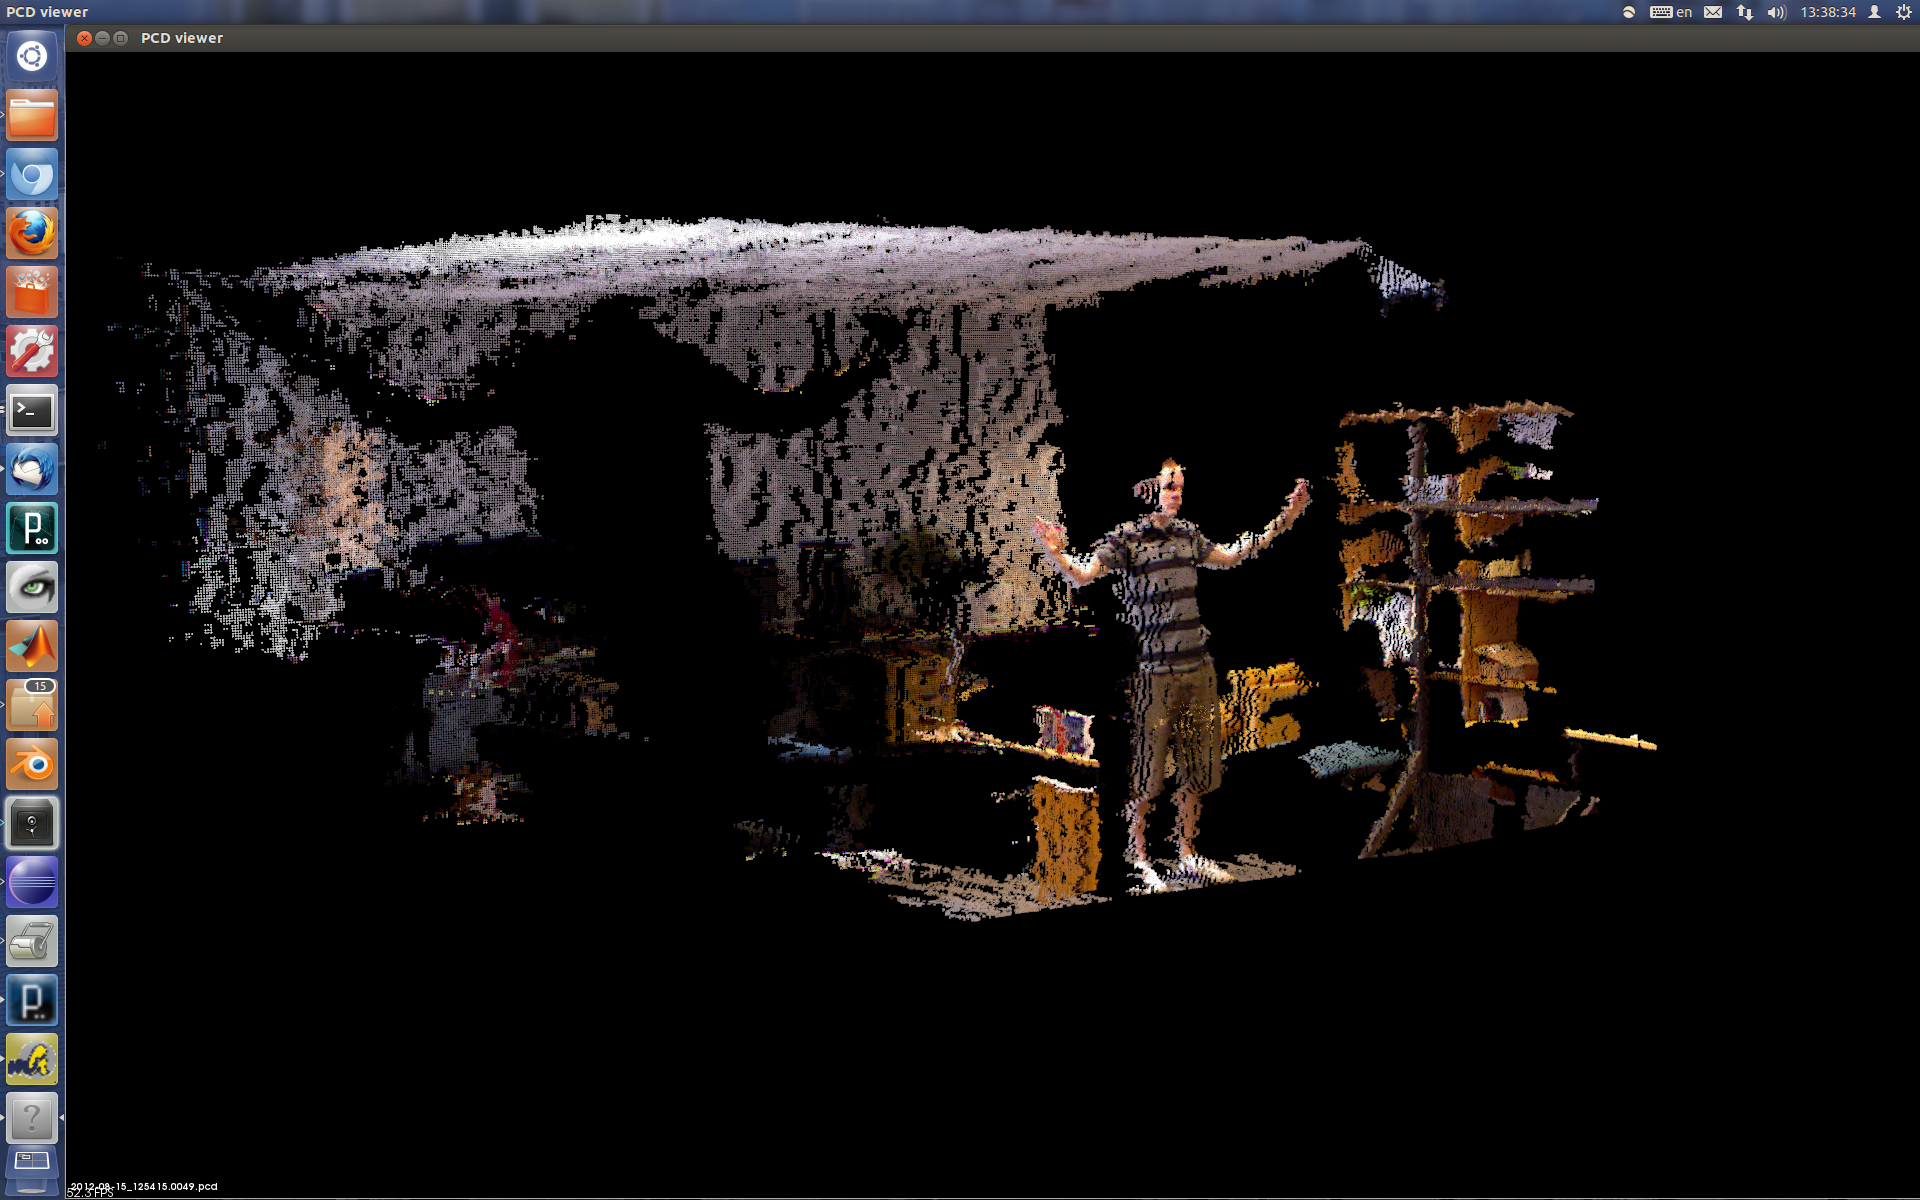
\includegraphics[width=\textwidth]{pcd-plain.png}
    \caption{A point cloud constructed from a single frame of Kinect data. The cloud is captured and saved in the PCD (Point Cloud Data) format that PCL uses \citep{pcdspec}. The viewer used is part of PCL.}
    \label{fig:pcd-plain}
\end{figure}

As we receive data from the sensor, we need a representation for it. Physically, the Kinect has two cameras: one RGB and one IR. The data received from the sensor is an 8-bit Bayer-filtered image and an 11-bit depth image computed onboard from the IR data; both have a resolution of 640x480 and a framerate of 30 fps. It is possible to request different resolutions or the raw IR image, but these are the most sensible choices. The drivers interpolate the Bayer image to get a 640x480 RGB image.

Converting the data to a point cloud allows more sophisticated processing than using the plain images. A point cloud represents the actual real-world geometry of the observation, allowing interpreting the point locations as vectors and using standard mathematics. Image-based algorithms do exist for some tasks and usually are computationally very efficient compared to algorithms operating on 3D point sets, but they tend to be very unintuitive.

The point cloud representation allows geometrical operations, one practical application of which is to render the data from another viewpoint as seen in figure~\ref{fig:pcd-plain}. This kind of 3D rendering with a freely moving camera was used to get acquainted with the data of Kinect. Looking at the point cloud data from Kinect in real time helps notice the kind of noise inherent to Kinect. The most evident types of errors in the data are:
%
\begin{description}
    \item[Jitter in depth measurements.] The depth of a single pixel in a static scene may seemingly randomly change between two or three values. Possible explanations for this are that the actual distance is between two possible discrete values, or that the point is almost at an edge and could be interpolated to be on either side. Very small differences in the observation then tip the balance.
    \item[Unaligned edges between the RGB and depth image.] Points in the foreground have the color of the background and vice versa. This happens near the edges, especially when an object is close to the sensor.
    \item[Missing points.] Because the depth is measured from disparities in a known laser pattern, the measurement cannot be made if a laser point cannot be reliably identified. This can be caused by occlusion, intensive light that covers the laser pattern, materials that absorb the IR wavelength used by the laser or areas that are so white that the IR sensor is saturated. As the result, the depth is set to a special value meaning it is unknown, and the point is not included in the point cloud.
    \item[Systematic errors.] Planes tend to be slightly curving---this means the conversion from depth image to world coordinates is inaccurate. This might be possible to overcome by careful calibration, but the error is small enough not to matter very much.
    \item[Biased normals.] Round objects seem flatter around the edges than they actually are. No measurements can be made where the surface is tangential towards the camera, and if there's a laser point on a nearly-tangential surface, its intensity is too low to be measured. Because depth values for most pixels are in fact interpolated from nearby measurements, and measurements can only be made on the relatively flat, camera-facing parts, objects seem to be flat. In other words, continuous depth variations in a strip of neighboring pixel are moderate at most.
\end{description}

Further experimentation on point clouds was made by compiling PCL and trying its examples. We made simple C++ code of our own utilizing PCL and OpenNI to grab a frame from Kinect and save it as a point cloud in the PCL file format. Point clouds captured this way could then be used as input for applications included in the PCL distribution. We examined the convex and concave hulls of point clouds to see if they might be useful. We tested fast mesh generation, which allows viewing an approximate surface of the Kinect view in real time, albeit with a lot of noise. We also compiled Kinfu and experimented with it, even making some changes of our own to it---more on that in sections \ref{kinfurig} and \ref{voxelgrid}. One bug in the PCL IO module was also found and fixed while writing our own code\footnote{See \url{http://dev.pointclouds.org/issues/812}}.

% TODO: more \bs{important} things done with PCL

\section{Body part segmentation}

\begin{figure}
    \centering
    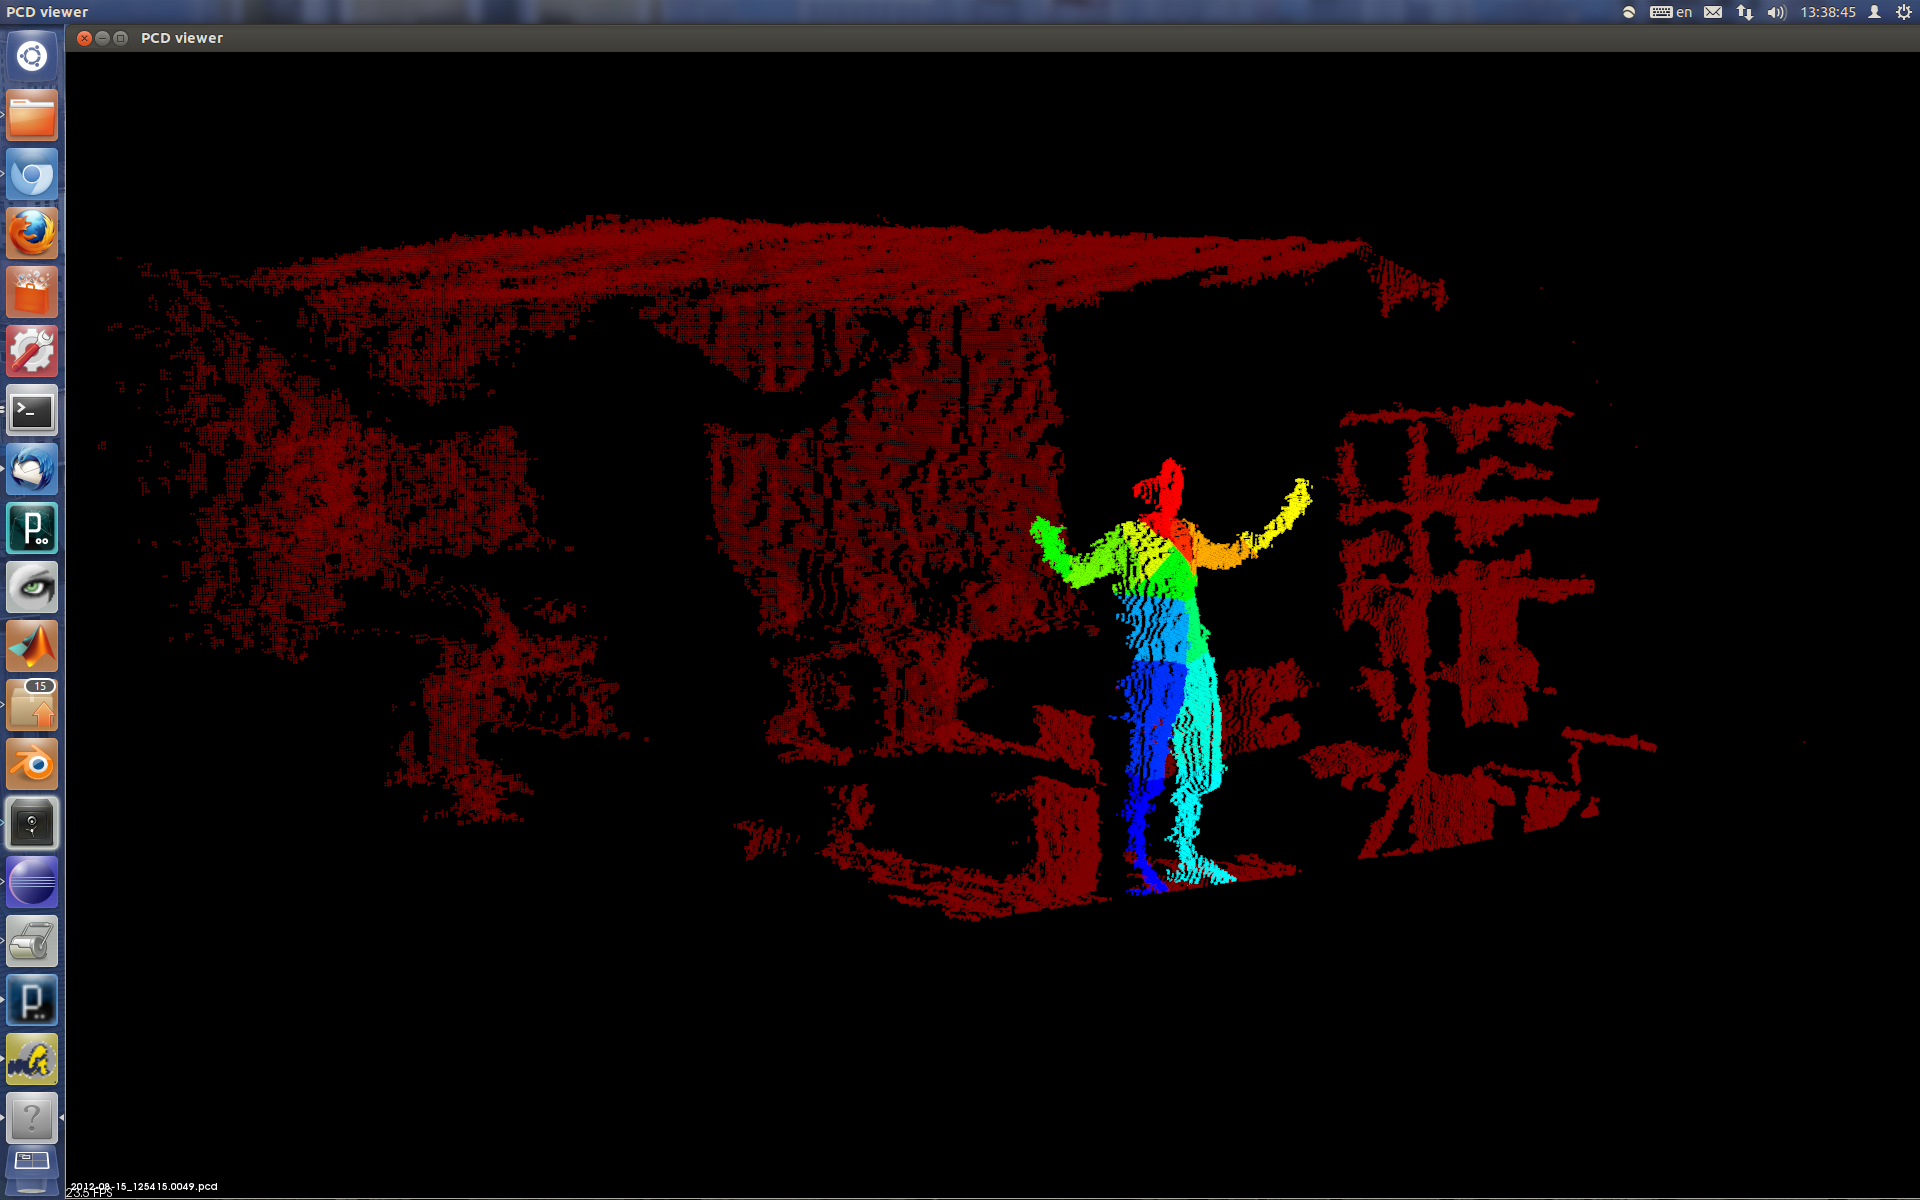
\includegraphics[width=\textwidth]{pcd-segmented.png}
    \caption{The same point cloud as in \ref{fig:pcd-plain}, with the user detached from the background and further segmented into individual body parts.}
    \label{fig:pcd-segmented}
\end{figure}

Before any attempts at human body reconstruction can be made, the body needs to be detected from the RGB-D image. % mention 'segmentation'

The NITE middleware for OpenNI \citep{NITE}
includes functions for person detection. Moreover, NITE has the capability to generate a skeleton representation of human users.

As the skeleton representation is available, we used it to aid in reconstructing the body model.

Using the skeleton data, we segment the point cloud according to body parts.

The body parts used were chosen according to what could be constructed from the joints provided in the NITE skeleton. Not all the joints are really joints in the human body, but they are treated as such in the simplified skeleton used by NITE. The joints that can be used are head, neck, torso, shoulders, elbows, hands, hips, knees and feet. NITE also has joints that exist in the API (Application Programming Interface) but whose positions are never updated: waist, collars, wrists, fingertips and ankles. 

Using these joints, we connected pairs to make bones and constructed the following body parts that we segment the point clouds to:
%
\begin{itemize}
    \item head and neck
    \item shoulders (left and right)
    \item lower chest
    \item abdomen (left and right)
    \item arm (left and right)
    \item forearm and hand (left and right)
    \item thigh (left and right)
    \item leg and foot (left and right)
\end{itemize}
%
Figure~\ref{fig:pcd-segmented} shows a body segmented according to these parts.

Body part segmentation as described was implemented in Processing using SimpleOpenNI. The method used is simple: for each point, compute the distance to all bones and choose the nearest one. This is not optimal, but could be improved later on. A possible optimization would be to only compute the distance to all bones for every $n$th point, and only consider the two closest points for neighboring points. Another one would be to project the bones to the image coordinates, and only compute 3D distances where the segmentation is not obvious in 2D.

After seeing the segmentation in action, we decided further study of the point clouds and skeleton positions frame by frame would be useful. To this end, we created a writer for the PCD file format used by PCL in Processing based on the released specification \citep{pcdspec}. This allowed making recordings of the point clouds that also contain body part index and RGB color as additional fields, something the file format has built-in support for. Furthermore, the PCD viewer included in the PCL distribution allows visualizing this---the colored body parts in figure~\ref{fig:pcd-segmented} were achieved with no modifications to the viewer application.

We also wanted the option to experiment with the original data: the skeleton joint positions. As the PCD format supported comments, we found it simplest to invent a header format that is interpreted as a comment in existing applications but could be read by software of our own. \fixme{TODO: format specification}

\fixme{TODO: example PCD listing?}

For experimentation, we created functions in MATLAB and Python (NumPy) for importing the plain-text PCD file format with our own skeleton extension. Some experimentation and plotting of the data was made in both, but generally PCL seemed to be a better platform for working with point clouds than either MATLAB or Numpy.

\section{Point cloud alignment}

The naïve approach to modeling uses data only from a single frame. However, this is unsatisfactory as in practice only less than a half of a human can be seen at once---when the front side is visible, the back is not. Another consideration is that the data tends to be noisy and inaccurate. Accumulating data over time makes it possible to remove some of the noise and improve accuracy.

To allow for combining data from multiple frames, the observations (point clouds) need to be aligned one way or another. Methods introduced in \autoref{literature.alignment} were available, each with their own trade-offs.

\fixme{TODO: write about alignment methods tested: PCL, CUDA EMICP + SoftAssign}

\subsection{Point cloud accumulation}

\fixme{TODO: figure}

Another approach was suggested by Klaus Förger from our research group, led by professor Tapio Takala. The idea is to gather point sets for different versions of each body part, depending on joint angles and orientation relative to the camera. Instead of trying to align point clouds, we would try to gather a lot of data and then use statistical methods such as averaging to avoid outliers.

This approach avoids the assumption that each body part is a rigid object by capturing separate data for different poses. This might allow for more accurate reconstruction, given sophisticated methods for modeling the body surface from the data. On the other hand, the amount of data is larger and finding a suitable method for creating the rigged mesh is more difficult. Ultimately, this approach would require further experimentation on how different surface reconstruction approaches work with the data.

A prototype of the accumulation code was made by Klaus. The implementation includes rendering of the posed skeleton, along with point clouds gathered with the current joint angles and orientations. Heuristics are used to omit unreliable observations, such as ones with fast movement. The video and depth images from Kinect tend to be slightly out of sync, causing errors relative to movement speed in the 3D coordinates of the points. This is most apparent in the edge between foreground and background.


\section{Mesh generation}

\fixme{Alternative approaches, including the following}

\subsection{Kinfu and automatic rigging} \label{kinfurig}

\begin{figure}
    \centering
    \begin{minipage}{0.49\textwidth}
        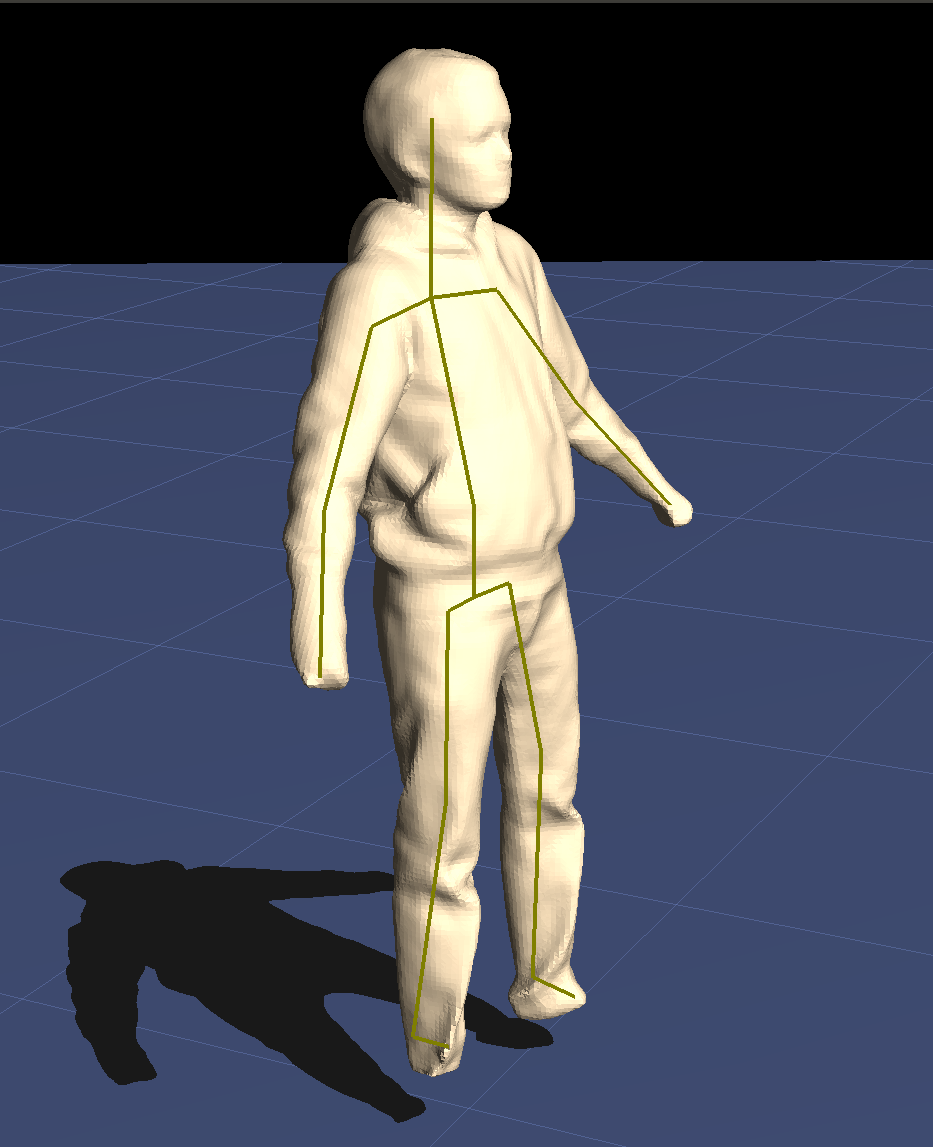
\includegraphics[width=\textwidth]{pinocchio-right}
    \end{minipage}
    \begin{minipage}{0.49\textwidth}
        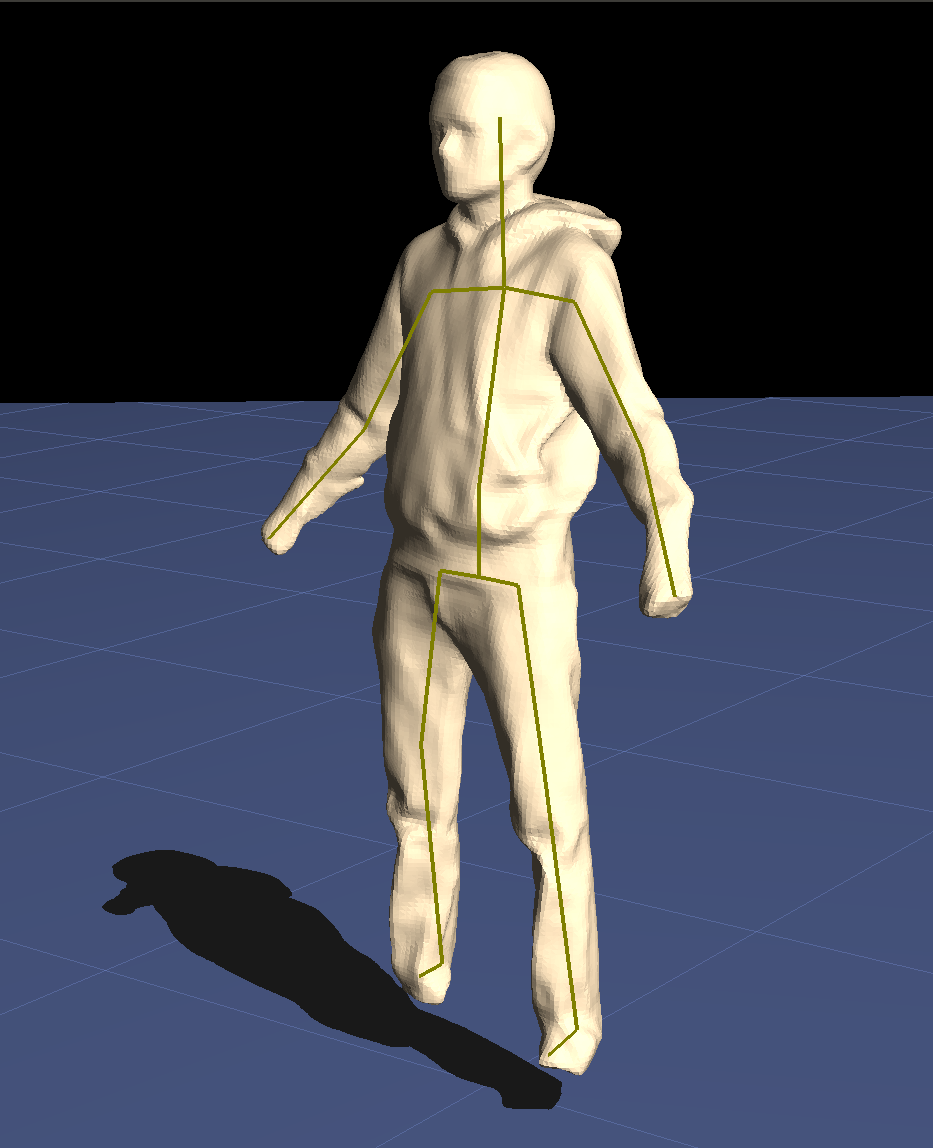
\includegraphics[width=\textwidth]{pinocchio-left}
    \end{minipage}
    \caption{The mesh scanned using Kinfu and rigged using Pinocchio. The skeleton is shown in olive.}
    \label{fig:hannu-front}
\end{figure}

\begin{figure}
    \centering
    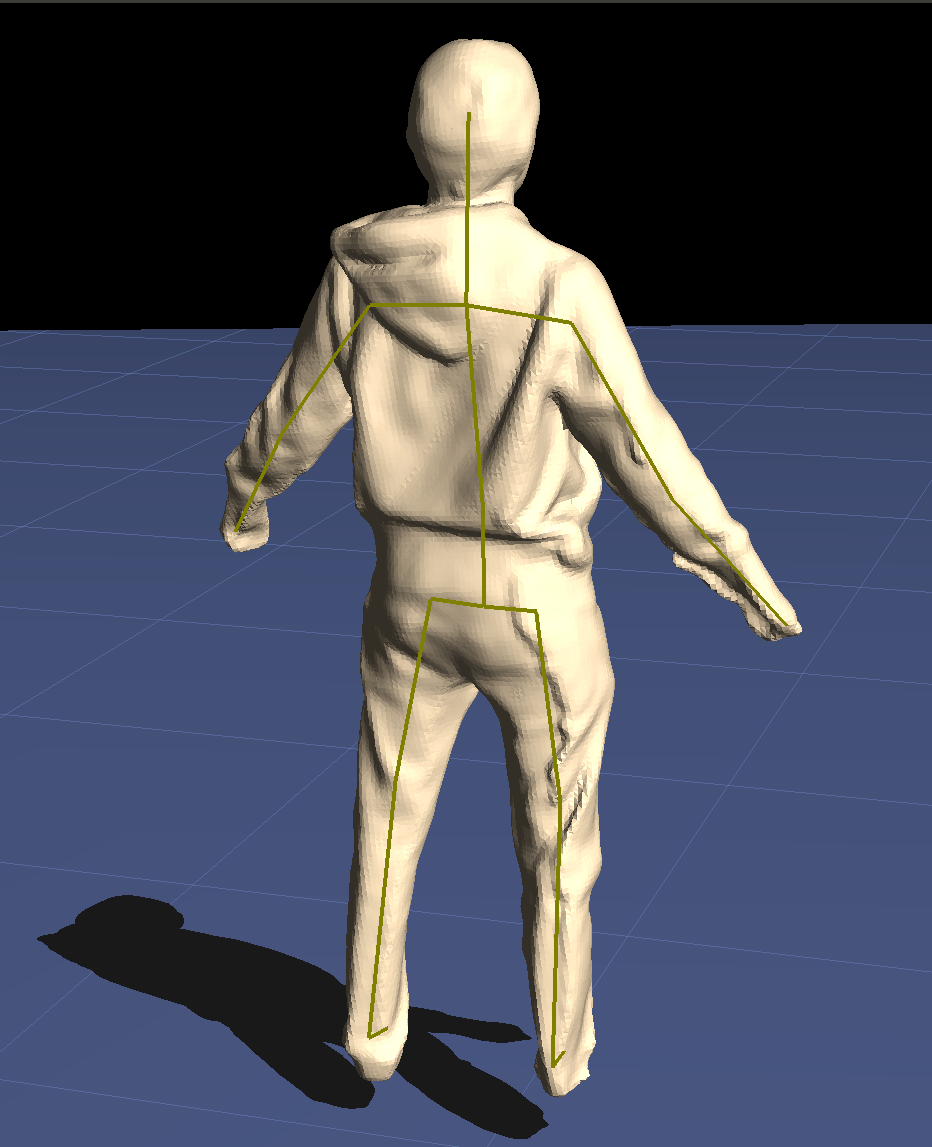
\includegraphics[width=\textwidth]{pinocchio-back}
    \caption{The back of the mesh shows inconsistencies in the right hand and leg.}
    \label{fig:hannu-back}
\end{figure}

\citet{charpentier2011accurate} shows how a rigged mesh model of the user can be made by manually aligning shots from different directions and then using an automatic rigging algorithm. \citeauthor{charpentier2011accurate} claims this approach would become very easy, if the KinectFusion system were available.

As the Kinfu implementation was available, this approach was tested in practice. The amount of manual work required turned out to still be surprisingly large.

The software needed for this approach are the KinectFusion system for scanning the mesh, a mesh editor for making necessary changes in the mesh and an auto-rigging software. We used MeshLab and Pinocchio for the latter two purposes, as \citet{charpentier2011accurate} had also successfully employed them. At the time of writing, Kinfu and Pinocchio needed to be compiled manually. Both have command-line interfaces that take a little getting used to; similarly, MeshLab's GUI (Graphical User Interface) is slightly confusing for a beginner.

The actual scanning requires two persons: one to be scanned and one to scan. The scanned subject needs to remain still while the other person carefully goes around them, slowly moving the Kinect so that as much of the body as possible can be seen. After this is done, the user presses a key to extract a mesh from the TSDF. This operation can only be completed if the GPU has at least 1.5 gigabytes of memory; otherwise, it's possible to change Kinfu source code to lower the TSDF resolution and recompile. The extracted mesh is then saved to disk by pressing another key.

The extracted mesh contains the subject and the surrounding area. The subject needs to be cropped for the automatic rigging. This requires manual mesh editing. In our test run, the full mesh was 140 MB in size and comprised some 5 million vertices and 1.5 million faces. Editing this mesh made MeshLab a bit sluggish on a high-end desktop computer\footnote{Intel Core i7-3770, 16GB RAM, SSD and an Nvidia GeForce GTX670.}. For comparison, the same mesh was imported in Blender, after which Blender became stuck for about a minute and then showed the mesh while remaining quite unusable.

After the mesh is cropped and only the human part remains, the actual editing can begin. Pinocchio needs a mesh that is closed and connected, and the one produced by Kinfu is very probably not. One possible approach to this problem is to uniformly sample a subset of the vertices and then use a mesh generation algorithm on those vertices. The downside is that some accuracy is lost, but on the other hand the regions with holes are nicely filled. Whatever approach is taken, it might take some trial and error to choose good algorithms and parameters. The computation is not instant, but not necessarily slow either, again depending on the exact methods used.

With this manual editing of the mesh finished, it is time to complete the automatic rigging using Pinocchio. In our tests, the first two tries failed because Pinocchio expects the mesh to be oriented in a certain way. This is not difficult to fix, but manual intervention is still needed at this stage.

Finally, Pinocchio successfully rigged the mesh and a walking animation of the user was seen on the screen---quite astonishing! Minor details such as slightly wrong placement of the shoulder joints made the animation a little unnatural, but the result as seen in figure~\ref{fig:hannu-front} still causes amazement. The mesh also has rough surface details, caused by drift in the camera position and lack of loop closure in Kinfu. This is shown in figure~\ref{fig:hannu-back}.

All in all, the amount of manual work required to create a rigged mesh from scratch was about an hour with some earlier experience of the tools. The process could possibly be automated, but implementing such an automatic system is far from trivial. The scanning phase would still necessarily need another person to move the Kinect around, and the time requirements would probably be around a minute for scanning and five minutes for processing. The method is thus feasible, but not as easy as \citet{charpentier2011accurate} suggests.

\subsection{Voxel grid} \label{voxelgrid}

One possible approach is to use a voxel grid similar to the one KinectFusion \autocites{newcombe2011kinectfusion}{izadi2011kinectfusion} uses. This allows generating meshes representing arbitrary shapes.

To evaluate the approach, a prototype was built on top of Kinfu\footnote{Kinfu is an open source implementation of KinectFusion \citep{newcombe2011kinectfusion}. It is included in the Point Cloud Library \citep{PCL}.}. Since the point clouds were already segmented by body part, it was possible to create recordings that only include a single body part. These recordings could then be played back and used as input for Kinfu.

The working hypothesis was that each body part could be treated as a static object, and that Kinfu should do quite well at modeling them. \fixme{Notably there's little difference between the camera moving} (as is the case in KinectFusion) and the object moving. If the background is filtered out, the result is similar. This made for the case that running the KinectFusion algorithm in parallel to each body part could give reasonably good results.

\fixme{TODO: tell what was done; changes to Kinfu, the steps taken to make data with only one limb}

In practice, Kinfu doesn't work well with isolated limb data. This has multiple causes. \fixme{1) For full-body scanning the whole user must obviously fit in the picture. At the VGA resolution that Kinect uses, this leaves few pixels per limb. 2) The depth resolution of Kinect is about 1--2 centimeters at a distance suitable for full-body scanning. 3) ICP only uses surface features for alignment, not color data. As the individual body parts tend to be quite smooth, this is a problem.}

\begin{figure}
    \centering
    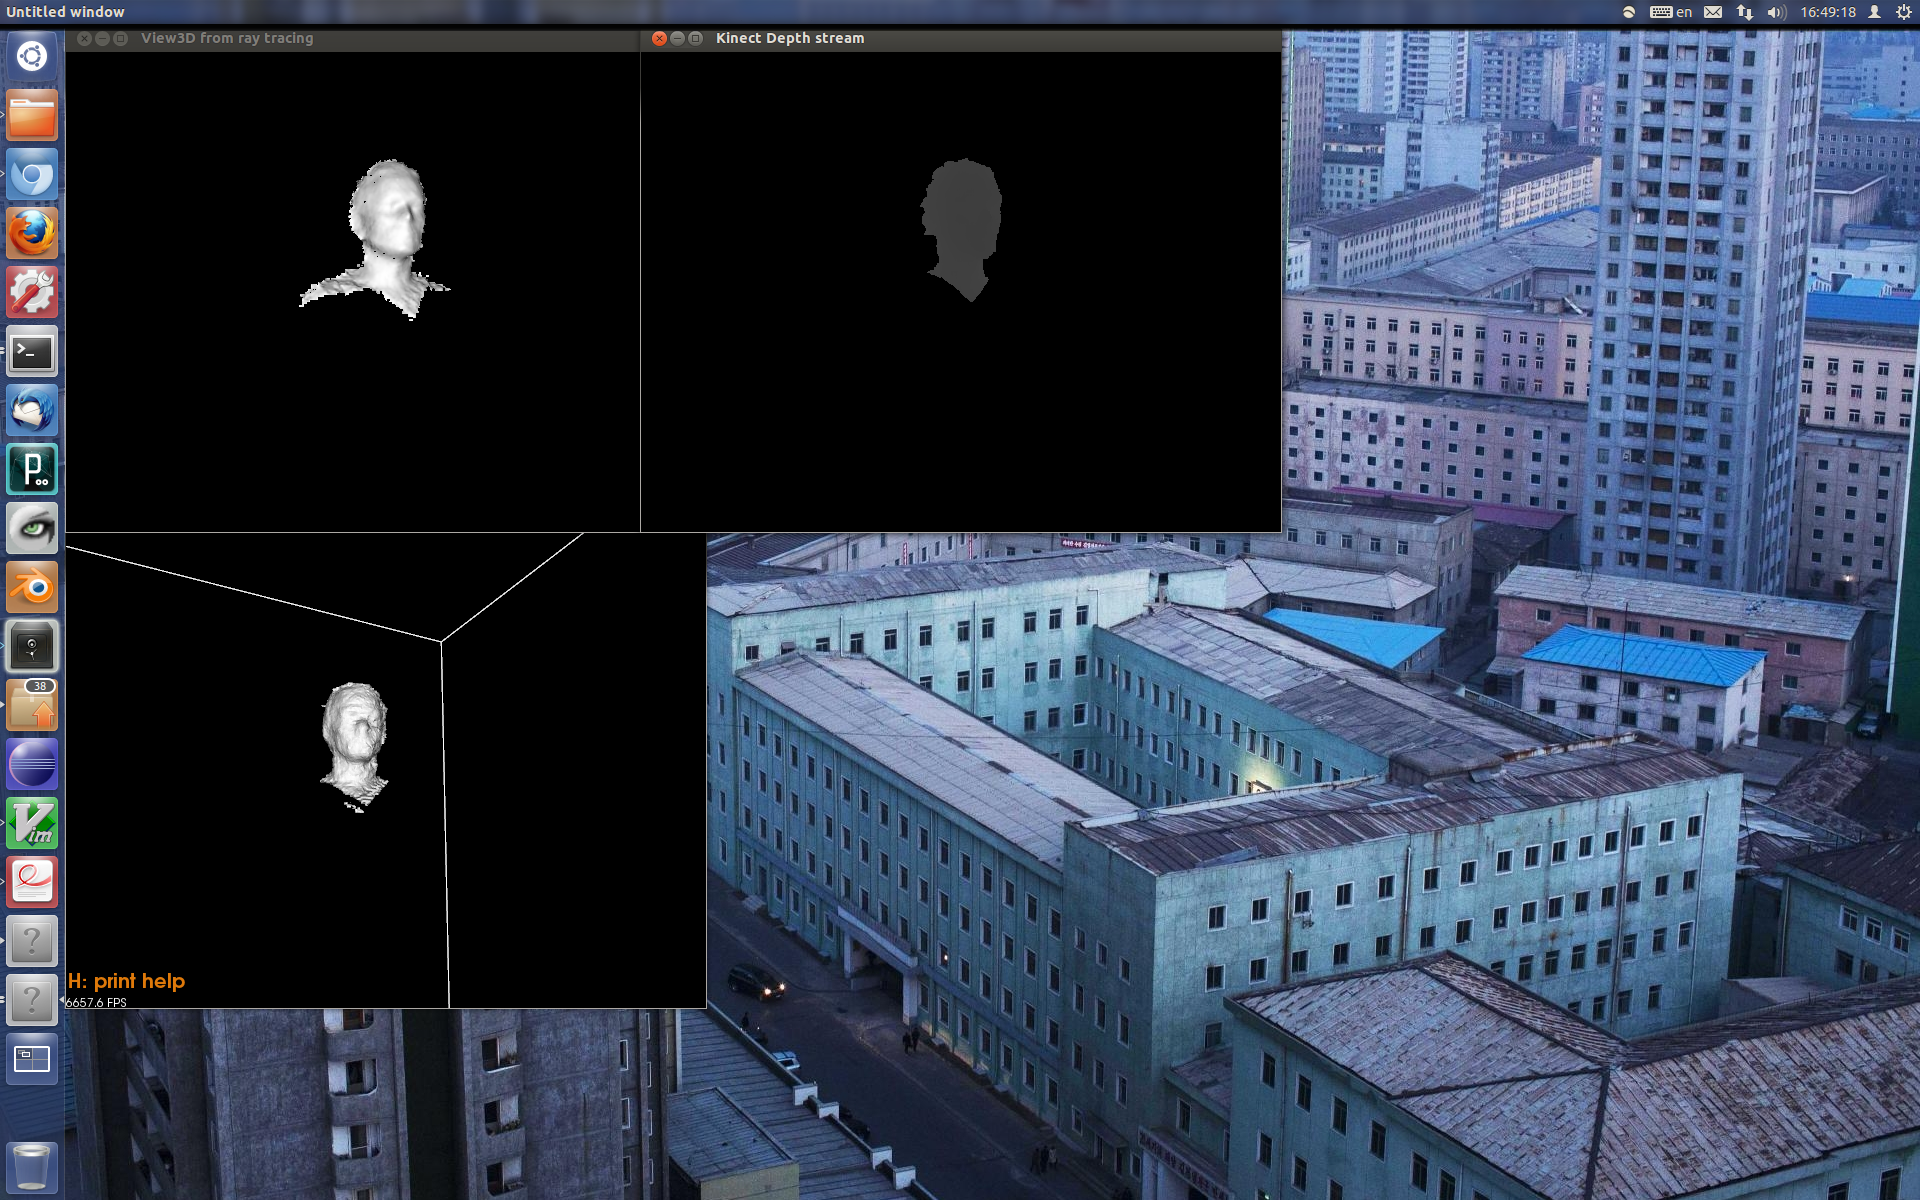
\includegraphics[width=\textwidth]{limbwise-head.png}
    \caption{Kinfu running on a view with only the head.}
    \label{fig:limbwise-head}
\end{figure}

\begin{figure}
    \centering
    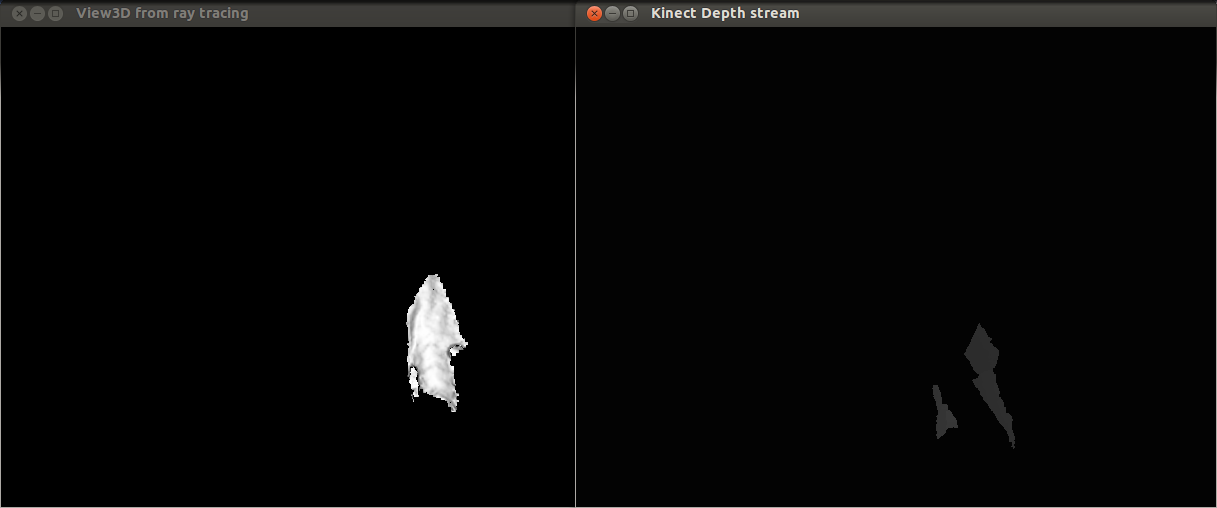
\includegraphics[width=\textwidth]{limbwise-arm.png}
    \caption{Kinfu running on a view with only the left arm.}
    \label{fig:limbwise-arm}
\end{figure}

\subsection{Parametric surfaces}

\fixme{TODO: cylinder man figure \label{fig:cylinders}}

\begin{figure}
    \centering
    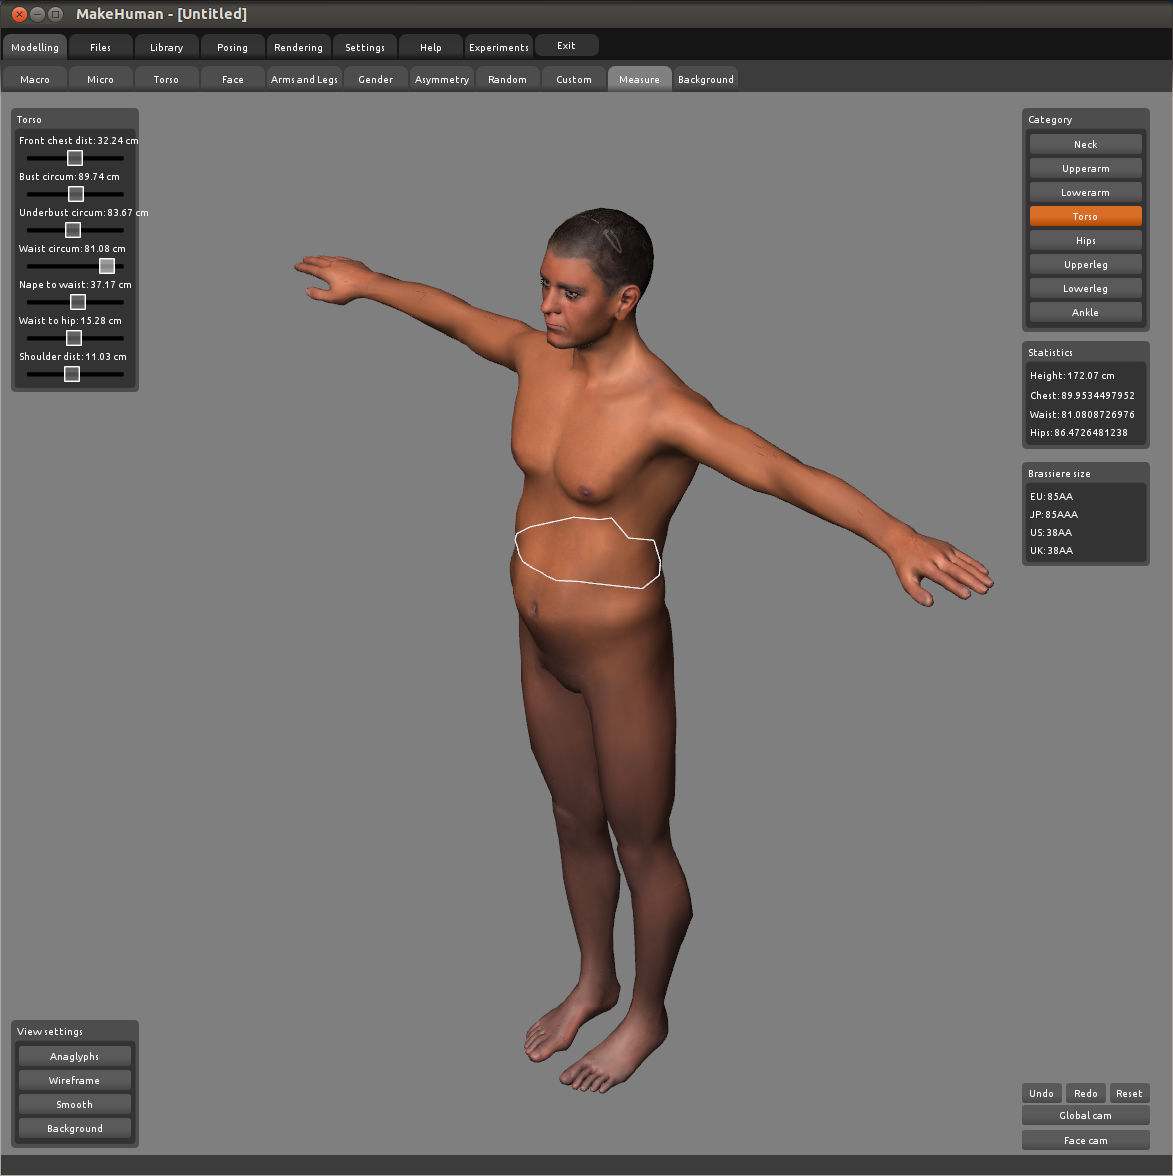
\includegraphics[width=\textwidth]{makehuman-measurement.png}
    \caption{MakeHuman with the Measurement plugin active. Waist circumference is selected. The white line shows where the circumference is measured.}
    \label{fig:makehuman-measurement}
\end{figure}

\begin{figure}
    \centering
    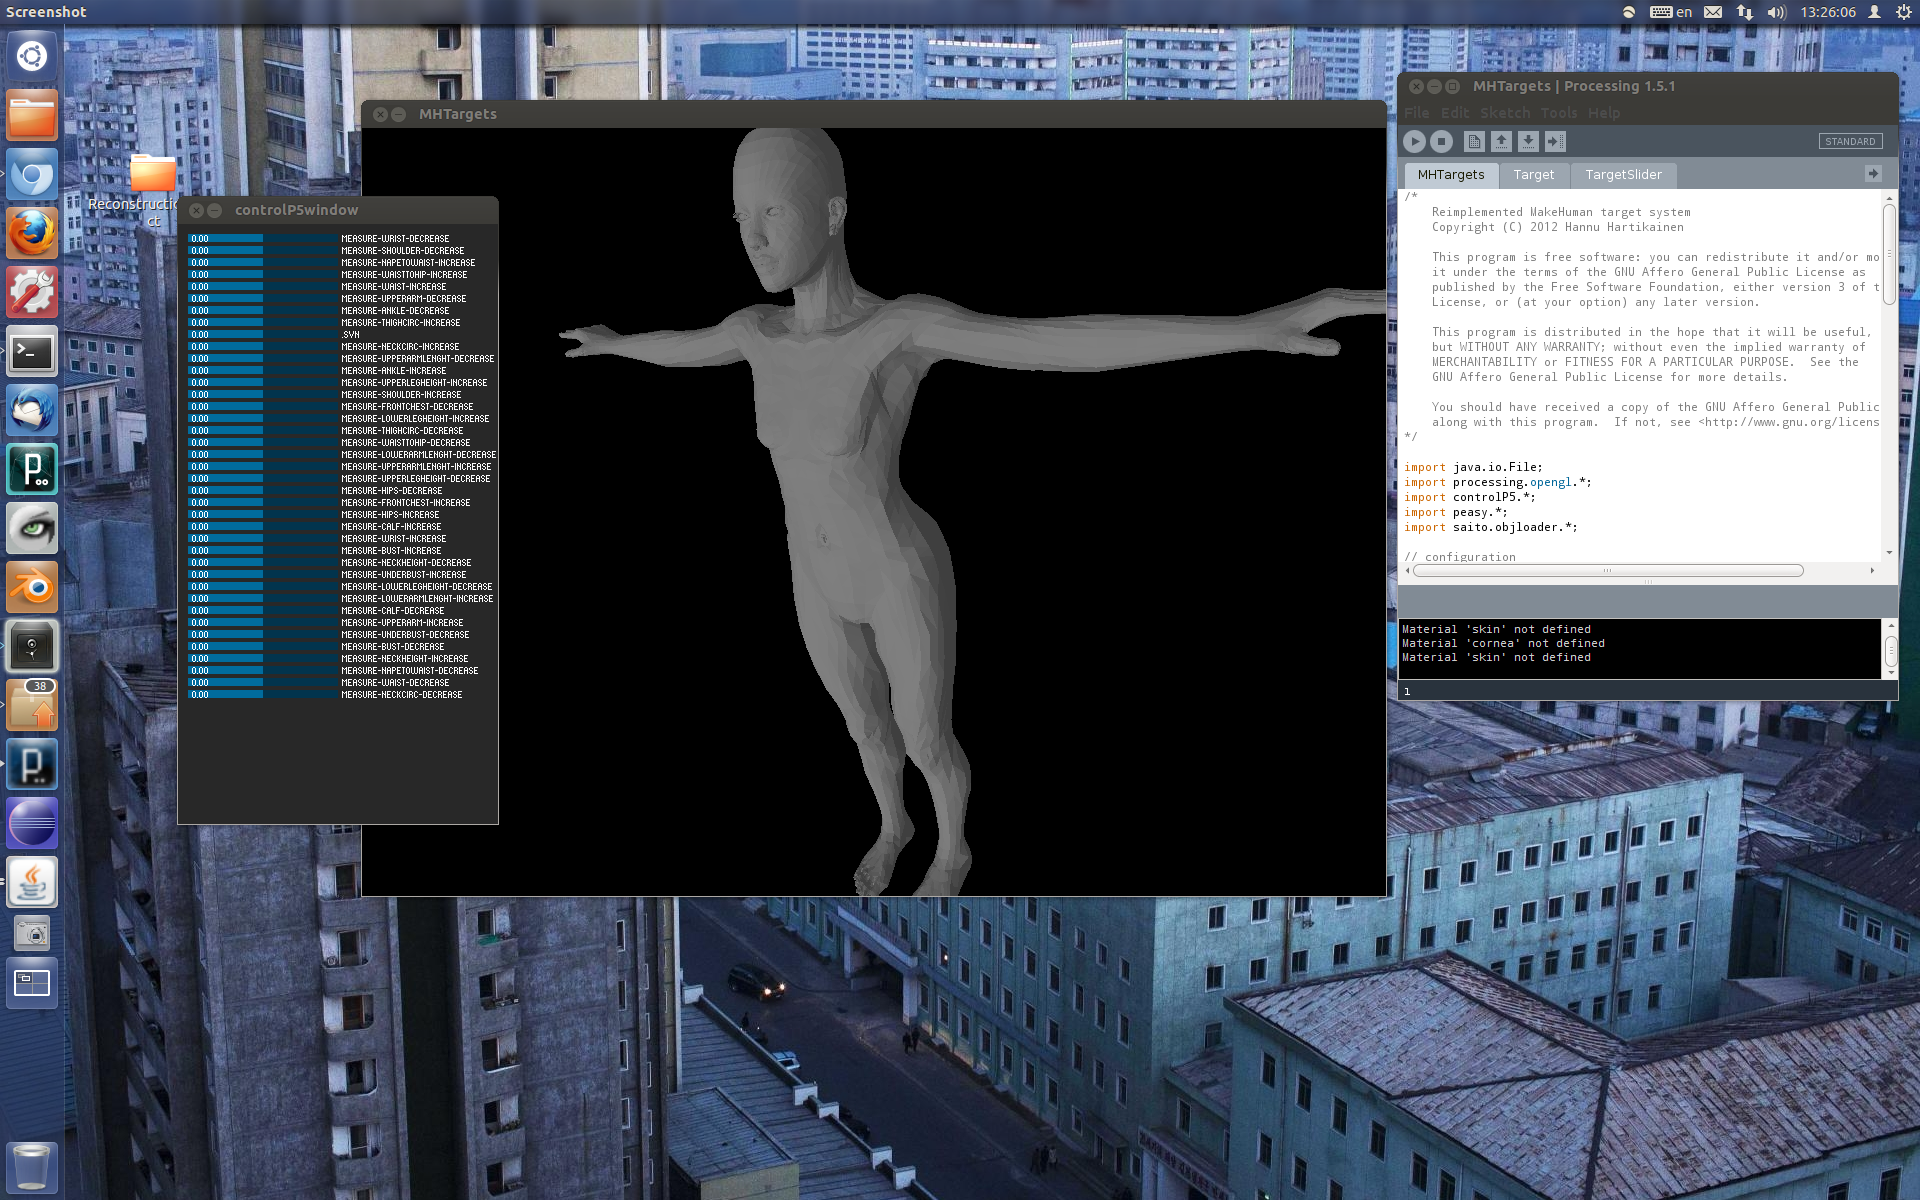
\includegraphics[width=\textwidth]{mhtargets.png}
    \caption{The reimplementation of the MakeHuman target system, showing the unmodified base mesh.}
    \label{fig:mhtargets}
\end{figure}

\begin{figure}
    \centering
    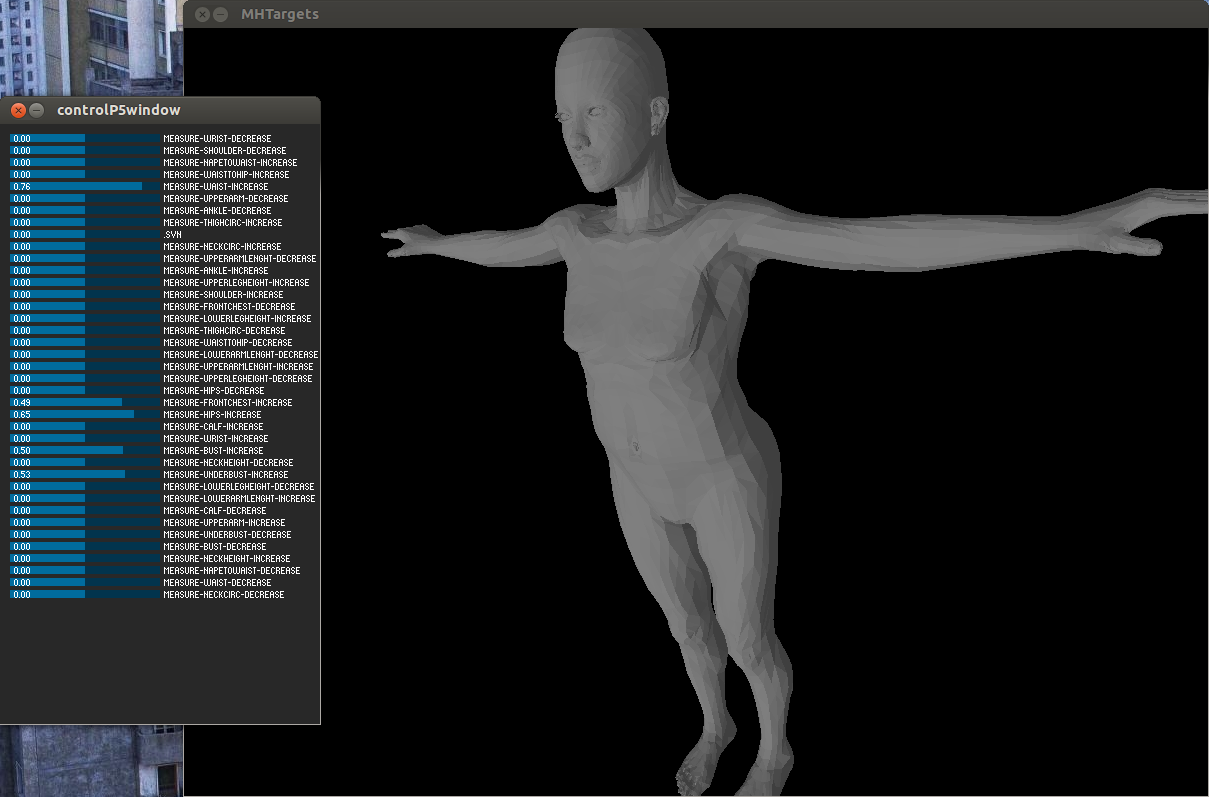
\includegraphics[width=\textwidth]{mhtargets-fat.png}
    \caption{The model in \ref{fig:mhtargets} with changed front chest, bust, underbust, waist and hip measurements.}
    \label{fig:mhtargets-fat}
\end{figure}

Another approach is to use the information readily available about the body parts being modeled. Instead of allowing arbitrary shapes, the space of possible shapes can be limited to what the body parts tend to look like.

As the very first prototype, a simple cylinder approximation was used. A cylinder was fitted to the point cloud of a body part, and colored according to its average color. This was good for testing the segmentation and getting a general idea of how accurate the skeleton is. Some corner cases were also found using this prototype. \fixme{elaborate...} \fixme{TODO: screenshot}

Obviously, a more human-like model was needed. The "cylinder man" could be usable as an avatar, and is certainly recognizable as human-like. But certainly its shape was nowhere near a real human body. Different simple shapes such as ellipsoids were considered. This would still have left the problem of connecting the body parts. A solution based on meta-blobs might have been feasible, but in the end this approach started to seem quite cumbersome. And still the accuracy would have left much to be hoped for.

The best parametric model for the purpose would then be something that already assumes the generic human shape, while allowing \fixme{exact} modifications to single body parts. The SCAPE model \citep{anguelov2005scape} used by \citet{weiss2011home} fits the description, but is not suitable for real-time evaluation. A more appropriate approach is taken by MakeHuman \citep{makehuman}, which uses a base mesh and has defined parameters that can be used to reshape different parts of the mesh.

Especially the Measurement plug-in in MakeHuman was promising, as it contained a good amount of parameters that mostly did not affect overlapping parts of the base mesh. For example, there are targets for arm length and circumference.

MakeHuman is still in development and at the time of writing was undergoing some large changes. It is not designed to be used as a library, either. Interfacing with other software thus seemed nontrivial. After some time tinkering with the MakeHuman implementation, it was decided that the data is important while the software can be replaced.

The \term{target} system in MakeHuman (see section \ref{literature.makehuman}) was implemented in Processing. The base mesh was also modified to only include the parts that should be drawn, while keeping mesh indices the same. The original base mesh contains octaedra representing some kind of control points, and for some reason, a dress that covers the body mostly.

\newtopic

Finding the correct target weights was still a problem. Different approaches were considered. The most naïve idea was to project the input point cloud to each body part and optimize the error between the point cloud and the mesh surface. This would require little knowledge of the effect of the targets, as different weights would be tried until good ones were found. By doing some good choices, such as optimizing length before circumference, this could be doable in real-time if the code was optimized.

Still, the idea of black-box optimization with expensive error computation on each iteration left questions about the implementation, and was not easy to begin working on. A better idea would be to make some measurements on the point cloud of a body part, and then make similar measurements on the mesh for each iteration of the optimization. This would significantly lessen the computational cost.

However, considering how the target system works, more deduction can be done beforehand. The magnitude of a target's effect is linearly defined by its weight. Therefore, if a measurement of the mesh is known for two values of a target weight, the weight matching another measurement value can be interpolated. This does require some assumptions: the targets must not overlap, the weights must be in reasonable limits (for example, the mesh must never clip itself) and the measurements must be linear.

\fixme{TODO: full follow-up}

\section{Texturing}

No actual implementation of texturing the mesh was made in this project, but possible approaches were considered. Of course, simple mixing of colors to get an overall color for each body part was tested for the simple ``cylinder man'' approach, and can be seen in figure~\ref{fig:cylinders}.

A simple way to get some more colorful details in the mesh would be to assign each vertex the color of the nearest point. This would allow visually representing some major details, such as the edge between a t-shirt and skin, or a colorful image on a shirt, or different color of face and hair.

For a better level of detail, an actual texture would be needed. Different approximations can be chosen to project the points to the surface (assuming they are not exactly on the surface, which they rarely are). One would be to use the surface normal coinciding with the point, and project the point on the normal's intersection with the mesh. Similarly, a normal of the bone could be used (where any line starting from the end of the bone and at over a 90 degree angle to the bone is considered suitable, too).

These approaches would work best by first finding the base color, as already implemented, and then adding local colors as appropriate. Each point should make a small ``splat'', and the different colors that coincide should be averaged. The choice of color space for averaging should be made based on practical evaluation, but at least averaging in RGB space seems to work reasonably well.

A confidence measure could be used, so that points far from the surface have a smaller effect on the final color. Practically a Gaussian function such as
\begin{equation*}
    e^{-x^2},
\end{equation*}
or more generally,
\begin{equation*}
    a e^{-b x^2} \mid a, b \in \mathbb{R}_+
\end{equation*}
could be used for the weight of a point as a function of its distance to the surface, and also to control the color intensity of the splat.

Another method of coloring the texture could be to pose the created model to correspond with silhouettes in the RGB images. Then the projection would be made through a camera ray from the image plane to the surface. This would practically be difficult to implement, as optimally the texturing should be done for previous frames using the current mesh. The texture segments from different frames should then be somehow stitched together.

One notable problem about using the RGB data for texturing are the non-uniform lighting conditions. Some pixels are in the shadow and too dark, while others are overexposed. This problem is very difficult to avoid, as it would require knowledge of the lighting and inverse computation of shading.

\section{Recording Kinfu trajectory}

\fixme{Can I fit this somewhere?}

Due to the work already done on Kinfu (see section~\ref{voxelgrid}) it was easy to make minor changes for recording trajectories. This proved useful in other research, which yielded one conference paper \citep*{tykkalavisapp} and one journal article \citep*{tykkalavcir}. Both are accepted to be published in 2013.
